\documentclass[11pt,twoside,a4paper]{report}


% ------- Enable UTF8 characters ------- %
\usepackage[utf8]{inputenc}
\usepackage[english]{babel}

\usepackage{marginnote}
% --------------- Math ----------------- %
\usepackage{amsmath}
\usepackage{amsfonts}
\usepackage{mdframed}
\newcommand{\dif}{\mbox{$\mathrm{d}$}}
\newcommand{\ohm}{\mbox{$\Omega$}}

% ------------- Figures & Tables -------------- %
\usepackage{booktabs}
\usepackage{graphicx}
\usepackage{caption}
\usepackage{float}
\usepackage{subcaption}
\captionsetup[figure]{singlelinecheck=false, margin=0pt,labelsep=space,labelfont=bf,textfont=it}
\captionsetup[table]{singlelinecheck=false, margin=0pt,labelsep=space,labelfont=bf,textfont=it}
\usepackage{epstopdf} %MATLAB eps (vector) figures

\usepackage{array}
\newcolumntype{x}[1]{>{\centering\let\newline\\\arraybackslash\hspace{0pt}}p{#1}}


% --------------- Color ---------------- %
\usepackage{color}
\definecolor{dkgreen}{rgb}{0,0.6,0}
\definecolor{gray}{rgb}{0.5,0.5,0.5}
\definecolor{mauve}{rgb}{0.58,0,0.82}


% --------------- Code ----------------- %
\usepackage{verbatim}
\usepackage{listings}
\lstset{
	frame				= lines,
  	language				= C++,
  	aboveskip			= 3mm,
  	belowskip			= 3mm,
  	captionpos			= t,
  	showstringspaces		= false,
  	columns				= flexible,
  	basicstyle			= {\small\ttfamily},
  	numbers				= left,
  	numberstyle			= \tiny\color{gray},
  	keywordstyle			= \color{blue},
  	commentstyle			= \color{dkgreen},
  	stringstyle			= \color{dkgreen},
  	breaklines			= true,
  	breakatwhitespace	= true,
  	tabsize				= 3,
  	xleftmargin			= 17pt,
  	framexleftmargin		= 17pt,
  	framexrightmargin	= 17pt,
  	framexbottommargin	= 5pt,
	framextopmargin		= 5pt,
	moredelim			= **[is][\color{mauve}]{@}{@}
}
\lstset{
	literate				= {~} {\raise.17ex\hbox{$\scriptstyle\sim$}}{1}
}


\lstdefinelanguage{pseudo}{
  sensitive=false,
  morecomment=[l]//
}
\lstdefinestyle{pseudo}{
  language     = pseudo,
  commentstyle = \color{dkgreen}
}



\DeclareCaptionFormat{listing}{\rule{\dimexpr\textwidth+17pt\relax}{0.4pt}\par\vskip1pt#1#2#3}
\captionsetup[lstlisting]{format=listing,singlelinecheck=false, margin=0pt,labelsep=space,labelfont=bf}

\renewcommand\lstlistingname{Listing}



% ----------- Page Layout ------------- %
\usepackage{fullpage}
\headsep = 24pt % spacing between header and text
\usepackage{fancyhdr}
\usepackage{lastpage}
\usepackage{paralist}
\fancyhf{}
\fancyhead[LE]{\slshape \rightmark} % section
\fancyhead[RE]{\thepage}
\fancyhead[RO]{\slshape \leftmark} % chapter
\fancyhead[LO]{\thepage}
\pagestyle{fancy}
\setlength{\headheight}{15pt}


% font
\usepackage[T1]{fontenc}

\usepackage{titlesec}
\titleformat{\chapter}[display]
{\normalfont\Large\filleft}
{\sc\chaptertitlename\ \Huge{\thechapter}\\%
\vspace{1.5cm}
\titlerule[1pt]}
{-20pt}
{\Large}[\vspace{2ex}{\titlerule[1pt]}]

\titleformat{name=\chapter,numberless}[display]
{\normalfont\Large\filleft}
{}
{0pt}
{\titlerule[1pt]
\vspace{2ex}%
\Large}[\vspace{2ex}{\titlerule[1pt]}]

\titlespacing*{\chapter} {0pt}{0pt}{40pt}   %% adjust these numbers
\titlespacing*{name=\chapter,numberless} {0pt}{0pt}{40pt}   %% adjust these numbers


\newcommand{\HRule}{\rule{\linewidth}{0.3mm}}
\usepackage{blindtext} %Lorem Ipsum replica

% -------- Table of Contents --------- %
\usepackage[titles]{tocloft}
\usepackage[toc,page]{appendix}
\setlength{\cftbeforesecskip}{0pt}
\setlength{\cftbeforechapskip}{7pt}
\setlength{\cftbeforetoctitleskip}{-20pt}



\makeatletter
\newcommand*{\currentname}{\@currentlabelname}
\makeatother
\newcommand{\Mathias}[1]{\todo[inline,author=Mathias,color=red!20]{\currentname: ~ #1}}

% -------- TikZ --------- %
\usepackage{tikz}
\usepackage{circuitikz}
\usepackage{tikz-timing}
%\input{timing}
\usepackage{pgf}
\usetikzlibrary{arrows,automata}
\usetikzlibrary{patterns}
\usetikzlibrary{shapes.geometric}

\usetikzlibrary{fit}
\usetikzlibrary{calc}
\usetikzlibrary{intersections}
\usetikzlibrary{backgrounds}

\tikzset{desc/.style={outer sep=0pt,inner sep=0pt,text centered,font=\scriptsize,fill=black!10}}

\newcommand{\texta}{Helpful\\ \tiny (to achieve the objective)}
\newcommand{\textb}{Harmful\\ \tiny (to achieve the objective)}
\newcommand{\textc}{\rotatebox[origin=r]{90}{\shortstack{Internal origin\\ \tiny (product\slash company attributes)}}}
\newcommand{\textd}{\rotatebox[origin=r]{90}{\shortstack{External origin\\ \tiny (environment\slash market attributes)}}}


% -------- To Do notes --------- %
\usepackage{todonotes}


%---------- URL ----------%
\usepackage{hyperref} % clickable references
\hypersetup{
    colorlinks,
    citecolor=black,
    filecolor=black,
    linkcolor=black,
    urlcolor=blue,
    pdfborder = { 0 0 0 }
}
\def\UrlFont{}

%\usepackage[numbers, square, comma, sort&compress]{natbib}

\usepackage[
  backend=bibtex,
  %style=alpabethical,
  citestyle=verbose%-tcomp
  ]{biblatex}
\bibliography{bibliography} 

\usepackage[hang,flushmargin]{footmisc}


\begin{document}

% --------- Title Page, Front Page --------- %
\setcounter{page}{1}
\pagenumbering{Alph}

\begin{titlepage}

%\newcommand{\HRule}{\rule{\linewidth}{0.5mm}} % Defines a new command for the horizontal lines, change thickness here

\center % Center everything on the page
 


%----------------------------------------------------------------------------------------
%	TITLE SECTION
%----------------------------------------------------------------------------------------

\HRule \\[0.4cm]
{ \huge \textbf{ Controlling multiple drones autonomously \\ inspired by birds ability to keep formation}}\\[0.4cm] % Title of your document

\HRule \\[1.5cm]

\includegraphics[width=0.4\textwidth]{University_of_Southern_Denmark-logo} \\
\textsc{\large \emph{University:} \\   University of Southern Denmark }\\[0.5cm] % Major heading such as course name
\textsc{\large \emph{Author:} \\ Mathias Mikkel Neerup }\\[0.5cm] % Minor heading such as course title

%----------------------------------------------------------------------------------------
%	HEADING SECTIONS
%----------------------------------------------------------------------------------------

\LARGE Bachelor Thesis\\[1.5cm] % Name of your university/college
 
%----------------------------------------------------------------------------------------
%	AUTHOR SECTION
%----------------------------------------------------------------------------------------

\begin{minipage}{0.4\textwidth}
\begin{flushleft} \large
\emph{In coorperation with:}\\
Jussi Hermansen \\
Info@viacopter.eu \\
Cottagevej 4  \\
3300 Frederiksvaerk \\
\end{flushleft}
\end{minipage}
~
\begin{minipage}{0.4\textwidth}
\begin{flushright} \large
\emph{Supervisor:} \\
Kjeld Jensen \\ % Supervisor's Name
kjen@mmmi.sdu.dk \\
Maersk Mc-Kinney Moeller \\
University of Southern Denmark
\end{flushright}
\end{minipage}\\[4cm]


% If you don't want a supervisor, uncomment the two lines below and remove the section above
%\Large \emph{Author:}\\
%John \textsc{Smith}\\[3cm] % Your name

%----------------------------------------------------------------------------------------
%	DATE SECTION
%----------------------------------------------------------------------------------------

{\large June 1, 2016}\\[3cm] % Date, change the \today to a set date if you want to be precise

%----------------------------------------------------------------------------------------
%	LOGO SECTION
%----------------------------------------------------------------------------------------

%\includegraphics{Logo}\\[1cm] % Include a department/university logo - this will require the graphicx package
 
%----------------------------------------------------------------------------------------

\vfill % Fill the rest of the page with whitespace

\Mathias{A bachelors thesis (15 ECTS) report from a single student should have a length no more than 35 
pages plus maximum 10 pages of appendices.}
\end{titlepage}

%\section*{Acknowledgement}
Throughout the project period my classmates has been at great help to discuss and generate ideas.

Especially thanks to the people listed below.
\begin{itemize}
	\item My supervisor Kjeld Jensen for giving solutions and help when needed.
	\item Developer of MarkerLocator Henrik Midtiby for helping me understand and adding functionality to his software.
	\item Friend Morten Albeck Nielsen for meeting once a week to help generating ideas, debugging, sparring and proof reading the thesis.
	\item Friends Mads Tilgaard Jensen, Eskild Andresen \& Michael René Andersen for listening to technical issues, evaluating solutions and carrying out tests.
	\item My girlfriend Anna Riisberg Soerensen for proofreading the thesis and understanding the time required throughout this project period.
\end{itemize}




% --------- Front Matter --------- %
\setcounter{page}{1} % Start counter at 1
\pagenumbering{roman}

\listoftodos
    \setcounter{tocdepth}{2}

\chapter*{Abstract}
\addcontentsline{toc}{chapter}{Abstract}
Until now drones keeps getting bigger and larger to carry bigger batteries with more capacity and to lift heavier payloads. This leads to drones getting less efficient, less responsive and gets more dangerous. Instead it has become popular to make drones smaller and increase the number of drones needed to solve a task. \\

(Materials \& methods) \\
This thesis describes how to make three drones follow a leader drone with a preprogrammed path as an example of drones cooperating. A Linux PC running MarkerLocator tracks each drones position and wirelessly transmits, using Xbee, the drones positions to all drones.The position of each drone is spoofed into the drone using the CAN-bus and thereby overwriting the onboard GPS. An outdoor test has been made using the onboard GPS to test the leader-follower algorithm in a bigger scale. A small PCB has been developed and mounted on each drone to route packages from the Xbee module to the CAN-bus of the drone and to measure the local altitude of the drone using a ultrasonic sensor. The PCB carries an AT90CAN128 as microcontroller which build-in CAN support making it obsolete to carry an external USB CAN-controller.\\


(Results -> discussion)\\
The accuracy of the vision based localisation is measured using a laser pointer pointing out the drones 2D position on the floor making it possible to measure the variance of the drones position. The leader-follower algorithm was also tested outside using the onboard GPS. The performance of the leader-follower algorithm is measured and discussed using plots that reveals the distance between the drones.\\

(Conclusion -> perspective)\\
It is shown that it is possible to implement the leader-follower algorithm using a vision and ultrasonic based positioning system. The distance between all drones when flying indoor was +/- 10 cm which is less than the maximum accepted error. It was possible to add 5 follower-drones without editing the code showing it is a generic system The system can further be used to indoor testing of navigation algorithms and explore the many possibilities drones has to offer. If drones at some point needs to fly indoor to help eg. Mobile robots navigating, vision might be a way to obtain a absolute indoor position for the drones.
\newpage
\chapter*{Preface}
\section*{Acknowledgement}
Throughout the project period my classmates has been at great help to discuss and generate ideas.

Especially thanks to the people listed below.
\begin{itemize}
	\item My supervisor Kjeld Jensen for giving solutions and help when needed.
	\item Developer of MarkerLocator Henrik Midtiby for helping me understand and adding functionality to his software.
	\item Friend Morten Albeck Nielsen for meeting once a week to help generating ideas, debugging, sparring and proof reading the thesis.
	\item Friends Mads Tilgaard Jensen, Eskild Andresen \& Michael René Andersen for listening to technical issues, evaluating solutions and carrying out tests.
	\item My girlfriend Anna Riisberg Soerensen for proofreading the thesis and understanding the time required throughout this project period.
\end{itemize}


\newpage
\renewcommand\contentsname{Table of Contents}
\tableofcontents
%\addtocontents{toc}{\vskip-70pt}
\newpage

\chapter*{Reading Guide}
\addcontentsline{toc}{chapter}{Reading Guide}
This thesis contains three parts.\\ \\
\textbf{Chapter 1} gives background information about the purpose of this project. It starts giving an overview of the topic and ends up focusing on why it makes sense to make the project and what other universities have done. It further contains related work,  problem statement, defined hypothesis and assumptions and limitations. A image of the final extension board can be seen to make it clear to the reader how the developed extension board and AutoQuad Ladybird drone looks\\ \\
\textbf{Chapter 2} describes materials and methods used in this thesis. It explains how and why the following design chooses where made concerning firmware as well as developed PCB. Each chapter starts with an introduction and ends with test results evaluating weather the choices made works or not.\\ \\
\textbf{Chapter 3,4,5} concerns showing, analyzing and discussing results. Evaluation of the design choices made throughout chapter 2 with respect to the hypothesis is summarized in the conclusion. \\


On figure \ref{fig:drone_with_arrows} the different parts used in this thesis are highlighted.

\begin{figure}[H]
    \center
    \includegraphics[width=0.65\textwidth]{graphics/m4_arrow.png}
  \caption{Ladybird M4 drone with developed extension board}
  \label{fig:drone_with_arrows}
\end{figure}


% --------- Main Matter --------- %
\setcounter{page}{1} % Start counter at 1
\pagenumbering{arabic}
%\chapter{Reading Guide}
%This thesis contains three parts.\\ \\
\textbf{Chapter 1} gives background information about the purpose of this project. It starts giving an overview of the topic and ends up focusing on why it makes sense to make the project and what other universities have done. It further contains related work,  problem statement, defined hypothesis and assumptions and limitations. A image of the final extension board can be seen to make it clear to the reader how the developed extension board and AutoQuad Ladybird drone looks\\ \\
\textbf{Chapter 2} describes materials and methods used in this thesis. It explains how and why the following design chooses where made concerning firmware as well as developed PCB. Each chapter starts with an introduction and ends with test results evaluating weather the choices made works or not.\\ \\
\textbf{Chapter 3,4,5} concerns showing, analyzing and discussing results. Evaluation of the design choices made throughout chapter 2 with respect to the hypothesis is summarized in the conclusion. \\


On figure \ref{fig:drone_with_arrows} the different parts used in this thesis are highlighted.

\begin{figure}[H]
    \center
    \includegraphics[width=0.65\textwidth]{graphics/m4_arrow.png}
  \caption{Ladybird M4 drone with developed extension board}
  \label{fig:drone_with_arrows}
\end{figure}

\chapter{List of Abbreviations}
\begin{table}[H]
\hspace{-9pt}	% Move table to match margin of text
\begin{tabular}{p{0.15\textwidth} p{0.825\textwidth}} % If needed to regulate, regulate both numbers so their sum equals: 0.975
 AQ		&	AutoQuad \\
\end{tabular}
\end{table}

\chapter{Introduction}\label{chp:Intro}
Drones are more and more used in different applications in different areas because they make it relatively easy to get a quick or more in depth overview of a situation. A less positive thing of the drones is the amount of energy they are capable of carrying. A drone designed with long time-flight flying in mind is capable of flying approximately 20 minutes depending on weather and payload. If the drone is equipped with a heavy camera or other kind of payload, then the flight time starts to decrease rapidly. So far the solution has been to increase the size of the drones to mount bigger batteries, but this might not be right way of doing it. Drones become less efficient, less responsive and gets more dangerous due to increase in weight.

By looking at the nature, one can easily see how small animals like ants and birds manage to cooperate and thereby build or move bigger things that they would not be able to do on their own. This way of small independent, decentralized units working together is called a swarm.\\

By making drones smaller, they get more efficient, their flight time increase and they get cheaper but of the cost of their ability to lift. Therefore it seems like an idea to make small drones cooperate to solve more complex tasks.\\

SDU is currently using a platform called AutoQuad which is supported by large and small drones. Solving a task as a swarm is complex, and is not in the scope of this project. This project intend to implement a Leader-follower principle inspired by birds flocking behaviour. The leader-drone will have a preprogrammed flight path and the follower-drones will have no knowledge about the flightpath. Each follow-drone will try to keep a distance of 50 cm within plus minus 10 cm to its neighbours and the leader-drone. A computer program will be written to control each drone and tell them where to go without colliding. This will be developed in an indoor controlled environment. Since GPS is unavailable indoor, this project will be using vision, e.g. Henrik Midtiby's MarkerLocator to get the location of each drone. When the Follow-leader has been implemented it should in theory work outside as well, though with larger distances due to GPS inaccuracy.

\subsection{Related Work}
In order to find relevant research about drones flying indoor, a few search phrases was conducted.
The following keywords were used to create different phases: Indoor, environment, swarm, localization, AutoQuad, quadrotor, mini UAV, test facilities, ETH, accurate, RTK, totalstation.
Based on the keywords a few papers was deemed relevant to the project and has been combined in order to give the reader an overview within the field of this project. \\

Developers of AutoQuad did previously try to implement RTKLib \footnote{http://www.rtklib.com} in AQ. Unfortunately they did manage to make it work as expected \footnote{Jussi Hermansen, owner of \url{http://ViaCopter.eu}}.\\

One of the big players within the field of indoor navigation and controlling multiple drones accurately is the university ETHzûrich and their Institute for Dynamic Systems and Modelling \footnote{\url{http://www.idsc.ethz.ch/research-dandrea/research-projects/aerial-construction.html}}. They have developed a test flying area they call "Flying Machine area" which provides facilities for doing prototype testing of new control algorithms \footcite{lupashin2014platform}. The FMAs dimensions is 10*10*10m and provides nets to protect people and mattresses to protect the drone  if a crash. The FMA has further been developed into a mobile installation to be used in demonstrations in Europe and North America. One of their demonstrations where used in a TED video about multiroters and their capabilities \footnote{https://www.ted.com/talks/raffaello\_d\_andrea\_the\_astounding\_athletic\_power\_of\_quadcopters}.
The multiroter usually used in the FMA is Ascending Technologies' Hummingbird with custom wireless communication and electronics. \\
They have build it as a module design in order to be easy to replace parts of their system by simulations and to make it scalable.
One of their modules is a copilot that implements an accident handler in case of user-code crashing or sending invalid commands to the drones.
They are using UDP multicast packets as communication between ground computation and flying objects. The use of UDP multicast packets between modules since to makes the system more simple but also to avoid the need of buffers to handle unsuccessful transmissions and retransmissions. \\
In order to detect the quadroters they are using a commercial motion capture system. Three reflective markers is mounted on each flying object in order to obtain attitude and position. They are using three cameras to reduce the risk of false positive even though two cameras would be enough to get a flying objects 6D position.\\
 
 
\cite{kang2015indoor} proposes a more simplistic approaches to do indoor navigation.
They use bluetooth 4 to communicate between their multiroter(Rolling Spider) and an android phone which controls the multiroter.
They have mounted a camera on the ceiling to detect the target and the flying multiroter.
By doing background subtraction they can detect where the drone is in the frame by subtracting the background from each frame \footcite{wikiBackgroundsubtraction}. 
By doing a convolution sum, the targets can be located. By analyzing the pixels around the location of the multiroter, they can get the heading. \\

\cite{sanchez2014system} proposes a framework to accelerate the process of prototyping multiroters behaviors. Their framework is designed for a swarm of drones to fly in a environment with obstacles. One of their design requirements is, that the framework should be highly decoupled from the application the researcher is testing in order to speed up the development process. 
Position estimates is obtain by using onboard IMU and optic flow. To avoid expensive motion capture systems they have used markers that can easily be recognized by cameras mounted on the drones to get a absolute 3D estimate. Each obstacle got a ArUco-marker \footcite{Aruco2014} that can be detected by the front camera mounted on the multiroter. \\
They have decided to use ROS as middleware to provide generic interfaces between the modules used in their framework. Different multiroters can be used as long they use the same interface. Communication between multiroters and ground station(if used) is done using WIFI. \\


The most common type of indoor localization is using vision where the camera is either mounted in the environment or where the drone is equipped with cameras to obtain position estimates.\\
\cite{stirling2012indoor} uses a different approach where they use a \textit{Robot Sensor Network} to map the environment.
The idea is that each drone can either be a beacon or explorer. Each drone alternates between these two states. Beacons stays still below the ceiling without moving while explorer flies around to unknown locations. Beacons emit IR light in order to triangulate beacons position.  Beacons detecting unexplored locations calls for explorer that will become beacons and so forth until the environment is mapped. To synchronize the beacons 2.4 ghz WIFI is used. When the environment is mapped, graph searching algorithms can be used to find a path through the environment.
\subsection{Problem Statement}
The current AutoQuad version does not support any other source of global positioning than the onboard GPS and thereby does not accurate support flying within 3 cm\footcite{stempfhuber2011precise}. For AutoQuad to be used in applications requiring high accuracy this functionality is needed. \\
RTK-GPSs are unfortunately very expensive especially when they are small enough to be mounted on a drone. In order to add this functionality to AutoQuad, an indoor environment needs to be created in case of code behaving unexpected. Instead of using RTK-GPS indoor, a indoor positioning system will be developed. This test environment might be used later on to test swarm, navigation and control algorithms

\subsection{Hypothesis}
If each drone’s 2D position is obtained using vision and spoofed into the drone using CAN, then it is possible for at least 3 drones to follow a leader drone with a preprogrammed flight path and keep a euclidean distance at 50 cm within plus minus 10 cm to the leader and its neighbours.


\chapter{Materials and methods}
\textit{This chapter concerns the most important parts about how this project has been implemented. It has been split into several sections.}

\Mathias{Less calculations on the drone, better to move to another computer/cluster with more power than the drone has available from its battery}
\Mathias{Image of camera and drone seen from the side. Show what happens to the drones position estimation when it drifts down/up}

\section{System architecture}
alright
\newpage

\section{AutoQuad extension board}
\subsection{Introduction}
This secion will go in depth about the extentionboard created as an addon to the AQ M4 board. The extentionboard was developed to act as a bridge between the PC and the CAN-bus using wireless communication.\\

The block schematic shown in figure \ref{fig:PCB_block} was created by the auther. It was then given to Carsten Albertsen who created the schematic and did rest of the creation of the PCB. Some time was spend learning how to program the AtMega and ESP8266 but also on debugging since there was an error in the ISP pins. Later on the author had to make a correction to the board since a pin on the ESP8266 that had to be connected to ground.
\\
\subsection{Block schmeatic}
\Mathias{Create schematic appendix}
\Mathias{Add GPS, WIFI, PCB, PC to forkortelses liste}
\Mathias{Thanks to Carsten Albertsen for PCB development}
\begin{figure}[H]
    \center
    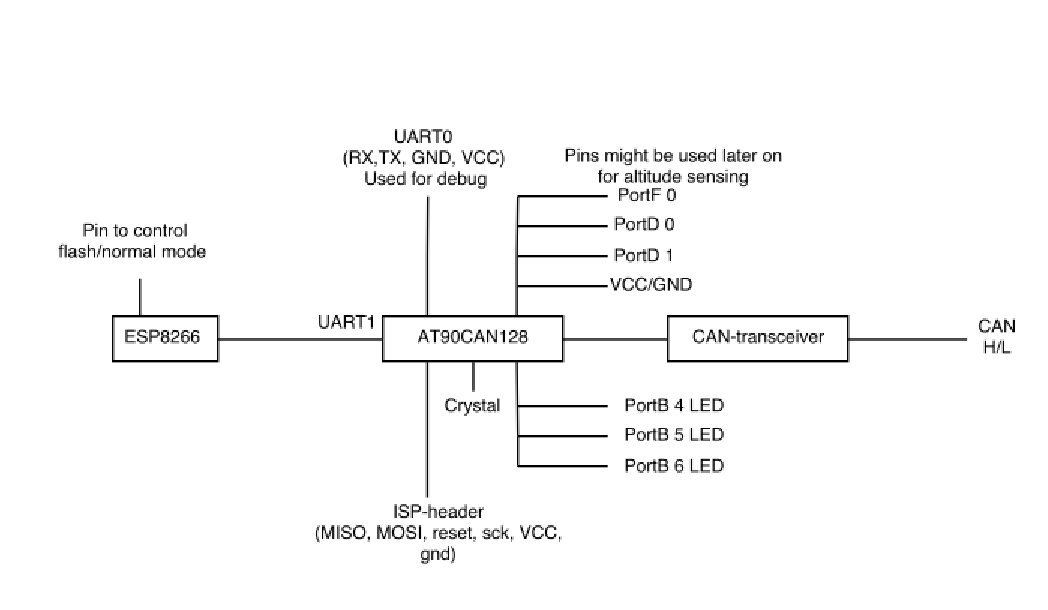
\includegraphics[width=1\textwidth]{graphics/PCB_block_v3.eps}
    \caption{Block schematic of the WIFI-extentionboard developed to AQ M4}
    \label{fig:PCB_block}
\end{figure}

\subsubsection{ATmega}
\subsubsection{Wireless communication module}
An important part of the hardware is the wireless communication used between the PC and the drones.
The wireless communication module has severel requirements it needs to fulfill in order to make the whole system work as expected. A comparison table has been made in table \ref{tab:compare_table_wireless_communication} to find the wireless communication module that is best suited for the task. \\
The following wireless modules where considered and compared.
\begin{itemize}
	\item \textbf{ESP8266}
\end{itemize}

ESP8266 is a generel purpose 32 bit SOC with integrated WIFI 802.11 b/g/n support and buildin TCP/IP stack. It can be setup its own access point or it can connect to an existing wireless network.
It runs at 80MHz and can be flashed with a custom firmware. 
The SOC is sold as modules with different pinouts and features such as extra flash memory \footnote{\url{https://www.olimex.com/Products/IoT/MOD-WIFI-ESP8266/open-source-hardware}} and different antennas.
The chip has been on the marked for about two years and costs approximately 7\$. 
It has been widely used in DIY-projects due to its low price and because it requires a minimum of network knowledge to get up and running.\footnote{\url{http://www.esp8266.com/} - 43.000 posts in forum} When the SOC is shipped, it comes with a preloaded firmware which either accepts AT commands or LUA scripting depending on the version of the module. These simple programming interfaces makes it quick and easy to interface the cheap. \\
This leads to a large community where most of the problems have been found and solved already. Arduino has been ported to ESP8266 which makes it even easier to get it up and running. Their official Arduino GitHub has 2125 commits on their master branch at the time of writing\footnote{\url{https://github.com/esp8266/Arduino}} \\

\begin{itemize}
	\item \textbf{EMW3165}
\end{itemize}
EMW3165 is a SOC much like the ESP8266 supporting 802.11 b/g/n WIFI with buildin TCP/IP stack. As with ESP8266 it supports setting up an access point aswell as connecting to an existing network. It has a Cortex-M4 $\mu$C which run at 100MHz. 
It supports custom firmware and can be aswell be bought as different modules with different pinouts and antennas.
It differentiates itself from the ESP8266 by its higher frequency its 5 volts compatible pins \footnote{\url{https://hackadaycom.files.wordpress.com/2015/07/emw3165.pdf}} which makes it easier to connect other hardware which run 5 volt without the need of a logic level shifter. It has been on the marked for only one year and costs approximately 9\$. Since it is a newer board than ESP8266 it has not been used in the same number of applications and thereby has a smaller community behind\footnote{\url{http://www.emw3165.com/} - 200 posts in forum }. Their most active GitHub has 147 commits on their master branch at the time of writing\footnote{\url{https://github.com/SmartArduino/WiFiMCU}}.

\begin{itemize}
	\item \textbf{nRF51822}
\end{itemize}
nRF51822 is also a SOC, but it is using Bluetooth instead of WIFI. The nRF51822 $\mu$C is implementing BLE which is a power efficient way of sending and receiving data. The chip supports broadcasting which could be used in this project. The $\mu$C can be bought as a standalone component or mounted on modules as the two other $\mu$Cs. Different modules offers different types of antenna connectors or buildin antenna on the PCB. It has not been possible to find an Arduino ported firmware that supports this $\mu$C. To write a firmware for the $\mu$C it has to be done using Nordic Semiconductor's proprietary SDK. 


\begin{itemize}
	\item \textbf{XBee}
\end{itemize}
XBee is a module that implements the Zbee standard. The Xbee modules work as a wireless serial connection. The Xbee modules supports mesh networking which means the modules by themself figure out which module is closest and makes the connection. This idea makes sense in this application since there will be multiple drones and one computer. If one drone gets too far from the PC, it can just connect to one of the other drones closer to the PC.\\
The Xbee solution is ready to use and requires a minimum of programming to get up and running. The modules also support GPIO for digital in and output and analog input.

\Mathias{ '\'footmotemark til at referere til samme fodnote flere gange}
\begin{table}[H]
	\centering
	\begin{tabular}{@{}|l|l|l|l|l|l|l|l|@{}}
		\toprule
		\textbf{Product} & \textbf{Size} & \textbf{Weight} & \textbf{Price} & \textbf{Documentation} &  \textbf{Range}  & \textbf{Score} \\ \midrule
		ESP8266   &  24x16mm\footnote{\url{https://www.mikrocontroller.net/attachment/243558/fcc\_11.pdf}} \hfill\{7\} & 1.5g\footnote{Measured by author on chemistry weight} \hfill\{8\} &   7.5\$\footnote{\url{http://www.seeedstudio.com/depot/ESP8266-based-WiFi-module-SPI-supported-p-2486.html}}    &   Great community \hfill\{9\}  &    ?    &                		\\ \midrule
		EMW3165   &  32x16mm\footnote{\url{https://hackadaycom.files.wordpress.com/2015/07/emw3165.pdf}} \hfill\{6\}  & 5g\footnote{\url{http://www.seeedstudio.com/depot/EMW3165-CortexM4-based-WiFi-SoC-Module-p-2488.html}} \hfill\{2\} &  9\$\footnote{\url{http://www.seeedstudio.com/depot/EMW3165-CortexM4-based-WiFi-SoC-Module-p-2488.html}}   &  Less available  \hfill\{3\}	        &    ?    &                		\\ \midrule
		nRF51822  &  18x10mm\footnote{\url{http://www.fanstel.com/Product/bluenor.html}} \hfill\{8\}  & 3g\footnote{\url{http://www.seeedstudio.com/depot/MDBT40P\%C2\%A0\%C2\%A0nRF51822\%C2\%A0based\%C2\%A0BLE\%C2\%A0module-p-2503.html}} \hfill\{0\}  &  7.5\$  & Ok documented\hfill\{2\} 	        &   30 M\footnote{\url{https://dl.dropboxusercontent.com/u/54939426/Fanstel_BT600.pdf}}  \hfill\{9\}     &                		\\ \midrule
		XBee      &  24.38x27.61mm \footnote{\url{http://www.digi.com/products/xbee-rf-solutions/modules/xbee-802-15-4\#specifications}} \{3\} & 3g \footnote{\url{http://www.digi.com/products/xbee-rf-solutions/modules/xbee-802-15-4\#specifications}} \hfill\{4\} &   25\$\footnote{\url{https://www.sparkfun.com/products/11215}}    &  Lots of DIY   \hfill\{9\}      &            91 M\footnote{\url{https://www.sparkfun.com/pages/xbee_guide}}  \hfill\{9\}  &                    \\ \bottomrule
	\end{tabular}
	\caption{Comparisontable used to compare different wireless 		communication modules}
	\label{tab:compare_table_wireless_communication}
\end{table}
\Mathias{vægt på ESP til 3 gram med link - det er hvad der er oplyst. Efterfølgende skrive at det er vejet til 1.51 gram(hen mod slutningen)}
The products compared in \ref{tab:compare_table_wireless_communication} are chosen to have approximately same specs. Onboard antenna, breakout for easy pin access.

\subsubsection{Pins}
A few pins where made available through solder pads for easy access if needed later on.

The following pins where available as solder pads:
\begin{itemize}
	\item PortF 0 - Alternative function as ADC, channel 0
	\item PortD 0 - Alternative function as interrupt, INT0
	\item PortD 1 - Alternative function as interrupt, INT1
\end{itemize}
In case the onboard baromter isn't accurate enough, an alternative distance could be used to measure the drones altitude with respect to the ground.
PortF0 has been made available since some distance sensors give output as an analogue value. 
An example of such sensor is an Infrared proximity sensor.\footnote{\url{http://www.sharpsma.com/webfm\_send/1208}} \\
As an alternative type of distance sensor, a ultrasoinc could be used such as HCSR04.
As output it gives a binary output with high-time proportional with the distance.\footnote{\url{http://www.micropik.com/PDF/HCSR04.pdf}}.
To detect the high-time, one of PortD1/0 would be useful. \\

Which type of sensor suits best as a distance sensor to provice altitude information to the drone is ouf of the scope of this report. The PCB has just been made ready to different types of sensors.

\subsubsection{Debug/ISP}
In the final schematic UART0 and ISP pins where combined in one pinheader for easy access through one cable. \Mathias{Refer to image of board}
To program the AtMega the ISP pins where required to be easy accessable. 
UART0 was made accessable to be used as debug and programming of the ESP8266 board.
The plan was to setup the AtMega as UART passthrough from UART0 to UART1.
Due to a mistake\footnote{The wrong pair of MISO/MOSI pins where made available in the ISP-header. The correct pair of MISO/MOSI is also RXD0/TXD0 as alternative function} in the final schematic, both UART0 and UART1 where made accessable trough the ISP/debug header. 
This ended up making it easier to program the ESP8266-board without using the AtMega as UART passthrough.

ESP noteS:
 - GPIO15 = bootmode, low for ...
 - GPIO0 = flash mode
 
 
 https://zoetrope.io/tech-blog/esp8266-bootloader-modes-and-gpio-state-startup

\newpage

\section{AutoQuad extension board firmware}
\textit{In this chapter the development of the firmwares running on the extension board is described. Different types of schedulers for the At90CAN128 is discussed and a scheduler is chosen and developed with the required functionality. The communication between PC and M4 is further described. At the end of each section a test is conduced in order to show if the code works as expected }
\subsection{Scheduler}
\textit{This capter concerns only the Atmega.  The ESP module will be descriped in section \ref{sec:esp_firmware}} \\
In order to have a timing on the At90CAN128 a scheduler was chosen and implemented.
The list below shows 3 different types of scheduler that was considered.
\begin{itemize}
	\item Real-time Operating System(RTOS) provides strict timing but at the cost of overhead. A RTOS runs task in a "parallel" environment. Each task runs in a loop and the RTOS scheduler will do context switching when needed. Using a RTOS requires mutexes and semaphores to protect shared resources which increases the complexity and amount of overhead
	\item Super-Loop provides no timing at all, but process data as fast as possible. It does not do any context switching and does not require mutexes or semaphores and  and thereby takes no overhead.
	\item Run-To-Complete(RTCS) scheduler is a mix of the two other schedulers. It works by waiting for a tick generated by a hardware timer and then starts executing all tasks from the beginning. The order of the task matters if there is dependency between the tasks but also to make sure the task requiring the most precise timing is at the beginning of the list of the tasks. All tasks have to be finished executing before the next tick is giving in order to avoid timing is ruined.
\end{itemize}
The RTCS was chosen since it provides timing without the overhead created when doing context-switching and the need of mutex and semaphores. It further reduces the code-complexity.\\

\Mathias{A little description about the scheduler implementation. Add tasks, and run the scheduler. Show how it waits for tick and the runs through all of the tasks that is in RUN state.}

It was decided to implement the code in tasks to make a low coupling between the functionalities. This makes it easier to maintain and expand later of if needed. The task diagram shown in figure \ref{fig:task_diagram_atmega} shows the tasks and how they do intertask communication.


\begin{figure}[H]
    \center
    \includegraphics[width=0.9\textwidth]{graphics/task_diagram.png}
  \caption{Tasks diagram showing overview of the running tasks on the At90Can128}
    \label{fig:task_diagram_atmega}
\end{figure}
A small description of each of the tasks is given below:
\begin{itemize}
\item \textbf{ is\_alive\_task} Toggles the green led to make sure the scheduler is running. In case of stack overflow, memoryleak or any other error, the Atmega will freeze and it will easily be detectable since the green led stops blinking
\item \textbf{ uart0\_tx\_task} Responsible of sending characters in the uart0\_tx queue.
\item \textbf{ uart0\_rx\_task} Responsible of checking if any characters in the uart-receive buffer is available. If any, put them into the uart0\_rx queue
\item \textbf{ uart1\_tx\_task} Responsibile as uart\_0\_tx\_task
\item \textbf{ uart1\_rx\_task} Responsibile as uart\_0\_rx\_task
\item \textbf{ can\_rx\_task} Responsible of checking if a CAN-message is available in the MOB. If any put them into the CAN\_rx\_queue
\item \textbf{ can\_tx\_task} Responsible of transmitting messages available in the CAN\_tx\_queue
\item \textbf{ aq\_node\_task} Responsible of registering the node when AQ boots.
\item \textbf{ task\_slip\_decode\_crc\_task} Responsible of removing SLIP characters and run CRC
\item \textbf{ aq\_spoof\_task} Responsible of converting and transmitting received GPS messages from uart1.
\end{itemize}
\Mathias{Add description of slip and crc task, maybe also spoof and node, not sure..}

\subsubsection*{Test of RTCS timing}
In order to test the timing of the scheduler, a led\_task was written. The task can be seen in code \ref{code:test_scheduler}
\begin{lstlisting}[language = c, caption = RTCS task used in timing test, label=code:test_scheduler]
void is_alive_task(uint8_t my_state){

	// Write to UART0
	UDR0 = my_state+'0';

	switch(my_state){
	case 0:
		INT_LED_ON_GREEN;
		INT_LED_OFF_RED;
		INT_LED_OFF_BLUE;
	    set_state( 1 );
		break;
	case 1:
		INT_LED_OFF_GREEN;
		INT_LED_ON_RED;
		INT_LED_OFF_BLUE;
	    set_state( 2 );
		break;
	case 2:
		INT_LED_OFF_GREEN;
		INT_LED_OFF_RED;
		INT_LED_ON_BLUE;

		// Set next state
	    set_state( 0 );
		break;
	}
	// Wait one second
	wait( 1000 );
}
\end{lstlisting}

The test was done by writing the current state of the task to UART0.\\ A python script were made that measures the time between each character received. The script can be seen in code \ref{code:test_rtcs_python}.
\begin{lstlisting}[language = python, caption = Python code used to measure time between received byte, label=code:test_rtcs_python]
#!/usr/bin/python
import serial
import time

ser = serial.Serial( port='/dev/ttyUSB0', baudrate=57600 )

t = time.time()
while True:
    char =  ser.read(1):
    print time.time() - t, ","
    t = time.time()

ser.close()
\end{lstlisting}
The output of the script were redirected to a file. After receiving 700 bytes the standard deviation and mean was calculated using matlab.
The mean is 1.0089 sec with a standard deviation of 0.0042 sec.

Part of the variance is caused by the inaccuracy of the timing on the PC running the python code. If a more accurate measure was needed, a scope could be attached to the $\mu$C's GPIO. Each time the scheduler enters the task the GPIO should be set high, and when it exists the GPIO should be set low. The scopes at SDU is capable of telling the variance of the off signal. \\
It can be concluded that the scheduler performs well.
\newpage

\subsection{Queues}
\subsection*{Test of CAN, queues}
In order to test CAN and queues, a task was written. The purpose of the task was to receive a CAN-message if any available from the queue and send the ID and data from the CAN message to a PC using UART.
The task used can be seen in code \ref{code:test_can_uart_task}.


\begin{lstlisting}[language = c, caption = Task used to test CAN, label=code:test_can_uart_task]
CAN_frame frame;
if(QueueReceive(&Queue_CAN_Rx, &frame)) {
	char ch;
	/* ID out uart0 */
	for(int i = 3; i >=0; i--){
		ch = ((frame.id >> i*8) & 0x000000FF);
		QueueSend(&Queue_Uart0_Tx,&ch);
	}
	/* ID end*/

	/* MSG out uart0 */
	for(int i = (frame.dlc-1); i >=0; i--){
		ch = ((frame.msg >> i*8) & 0x00000000000000FF);
		QueueSend(&Queue_Uart0_Tx,&ch);
	}
	/* MSG end */

	/* End of line */
	ch = '\r';
	QueueSend(&Queue_Uart0_Tx,&ch);
	ch = '\n';
	QueueSend(&Queue_Uart0_Tx,&ch);
}
\end{lstlisting}
The command used to send CAN-messages can be seen in code \ref{code:bash_send_can}.

\begin{lstlisting}[language = bash, caption = Task used to test CAN, label=code:bash_send_can]
while true; do sleep 1; print $(date); cansend can0  1DEADBEF#FEDCBA9876543210; done
\end{lstlisting}
The command sends a CAN-message using a connected PEAK-CAN adapter. It sends a message each second and prints out the date to make it clear when it is sending a message.\\ \textit{1deadbef} is the 29 bit ID and \textit{fedcba9876543210} is the 64 bit data. \\


The command used to show the received HEX values can be seen in code \ref{code:xxd}

\begin{lstlisting}[language = bash, caption = Command used to get UART messages, label=code:xxd]
cat /dev/ttyUSB0 | xxd -c 14 
\end{lstlisting}
Cat reads from /dev/ttyUSB0 and pipes its output to xxd where it is shown in HEX.\\ -c is number of columns which is 14 due to 4 ID bytes, 8 data bytes and 2 as newline.\\

The result can be seen in figure \ref{fig:can_recv_output}.
\begin{figure}[H]
    \center
    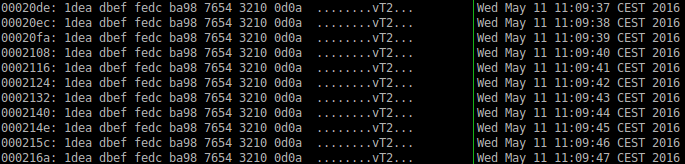
\includegraphics[width=1\textwidth]{graphics/xdd_can_test.png}
  \label{fig:boat1}
  \caption{Left shows output from command \ref{code:xxd} and right shows command \ref{code:bash_send_can}}
\end{figure}
It can be seen that the received ID and data is \textit{1deadbef} and \textit{fedcba9876543210} respectively.\\
\textit{0d0a} is \textbackslash r and \textbackslash n respectively.


\newpage
%\subsection{Tasks}
%\input{tasks}
%\newpage

\subsection{Wireless communication}
\subsubsection*{Communication flow}
\input{communication_flow}


\newpage
\subsection{CAN}
\subsection{Introduction}
In order to spoof the onboard GPS, the CAN-bus was chosen as input to AQ. 
The CAN-bus is already implemented and widely used on a ViaCopter drone to communicate between AQ and hardware like ESCs, PDB etc. Much time was spend reading through the source code and trying to figure out how the protocol works.
The developers behind AQ says, that the code is the documentation and thereby have not written any real documentation. \\
Figuring out how it works was done using debugging utilities such as breakpoints and looking at the content of the different memory locations in CrossWorks.
To further investigate the protocol a PEAK-CAN adapter were connected to a Ladybird drone and several python scripts were developed to send and receive messages from AQ. \\
The author did not go into details about messages used between AQ $\leftrightarrow$ ESC's and AQ $\leftrightarrow$ OSD.\\


\subsection{CAN Protocol description}
A Peak-CAN adapter were used throughout the project. It supports High-speed ISO 11898-2\footnote{\url{http://www.peak-system.com/PCAN-USB.199.0.html?&L=1}} which is a standard that states the properties of physical layer. 
Its max speed is 1 mbit which is the speed AQ uses to communicate on the CAN-bus. 
AQ uses CAN 2.0B which has 29 identifier bits.
AQ is not using an existing protocol on top of ISO 11898-2. The developers created their own to suit their needs.\\

\subsubsection{Identifier bits}
A Generic look at a AQ CAN messages can be seen in table \ref{tab:can_identifier_bits}.
The normal function of the identifier bits is the priority of the messages.
A CAN controller can then be setup to only allow certain messages to be processed depending on their identifier bits.
The identification bits has been split up in AQ to contain information about the sender, receiver etc. Which is not normally saved information in a CAN message.
\input{modules/Can-description.tex}

\subsubsection{Logic Communication Channel}
LCC is the priority of the message. 
To understand how LCC works, one needs to look into CAN arbitration.
As stated in ISO-11898-2, a 0 is the dominant bit and a 1 is the recessive bit.
The example in figure \ref{tab:can_arbitration} shows two nodes each transmitting a packet.
The arbitration only happens during the transmission of the identifier bits.
In the example on bit 8, Node 16 losses the arbitration and stops transmitting.
Node 15 keeps transmitting its packet because it has lower identifier bits and thereby higher priority.
\begin{figure}[H]
    \center
    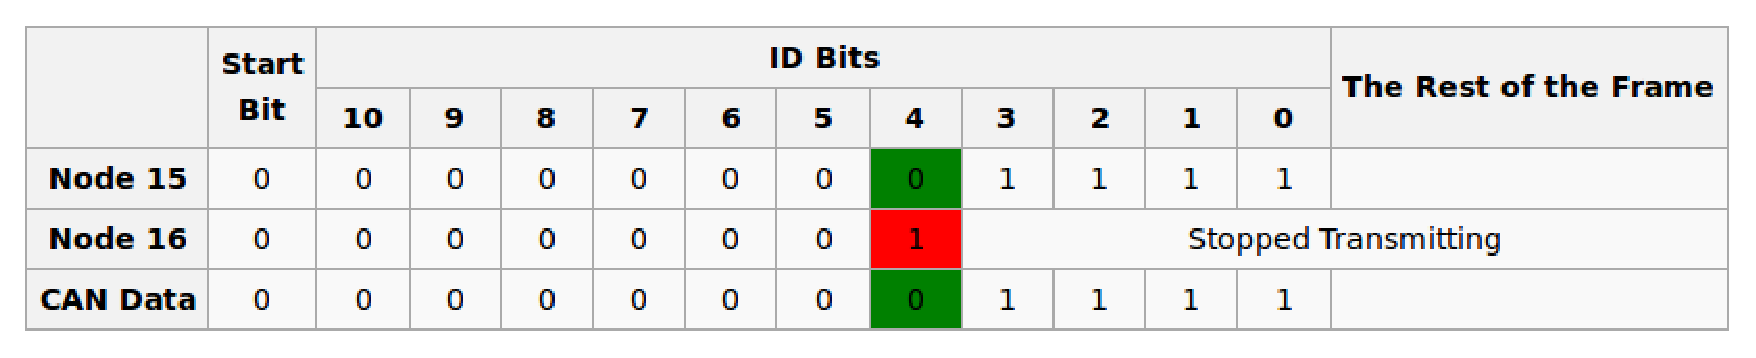
\includegraphics[width=1\textwidth]{graphics/can_arbitration.eps}
    \caption{Example of CAN arbitration where node 15 has the lowest ID and thereby highest priority}
    \label{tab:can_arbitration}
\end{figure}
\newpage
LLC in a message can take one of the defines in code \ref{code:llc_defines}
\begin{lstlisting}[language = c, caption = LLC defines, label=code:llc_defines]
#define CAN_LCC_EXCEPTION   ((uint32_t)0x0<<30)
#define CAN_LCC_HIGH        ((uint32_t)0x1<<30)
#define CAN_LCC_NORMAL      ((uint32_t)0x2<<30)
#define CAN_LCC_INFO        ((uint32_t)0x3<<30)
\end{lstlisting}

\begin{table}[H]
\centering
\caption{Table showing the 4 types of priority in AQ}
\label{my-label}
\begin{tabular}{|l|l|l|}
\hline
\textbf{Name} & \textbf{Value} & \textbf{Priority (lowest first)} \\ \hline
EXCEPTION     & 0000           & 0                 \\ \hline
HIGH          & 0001           & 1                 \\ \hline
NORMAL        & 0010           & 2                 \\ \hline
INFO          & 0011           & 3                 \\ \hline
\end{tabular}
\end{table}

\subsubsection{Target Type}
Target type can either be “node” or “group” depending on if the receiver(s) is one or more nodes. 
\begin{lstlisting}[language = c, caption = Target type defined in AQ, label=code:target_types]
#define CAN_TT_GROUP        ((uint32_t)0x0<<29)
#define CAN_TT_NODE         ((uint32_t)0x1<<29)
\end{lstlisting}
The GROUP is used when AQ sends its reset-msg upon startup.\\
When the authors node send a sensor-measure to AQ it will be of type NODE.
\subsubsection{Function ID}

Function ID describes the function of the CAN message. If it is a PING, ACK, NACK, etc.
It simply states the function of packet so the receiver node knows what to do with the message.
Different types of functions can be seen in code \ref{code:function_defines}
\begin{lstlisting}[language = c, caption = Excerpts from AQ's list of function defines, label=code:function_defines]
#define CAN_FID_RESET_BUS		((uint32_t)0x0<<25)
#define CAN_FID_ACK				((uint32_t)0x1<<25)
#define CAN_FID_REQ_ADDR		((uint32_t)0x7<<25)
#define CAN_FID_GRANT_ADDR	((uint32_t)0x8<<25)
\end{lstlisting}

Table \ref{tab:fid_descriptions} describes the FIDs shown in code \ref{code:function_defines}.
\begin{table}[H]
\centering
\caption{Descriptions of the FIDs mentioned in code \ref{code:function_defines}}
\label{tab:fid_descriptions}
\resizebox{\textwidth}{!}{%
\begin{tabular}{@{}|l|l|@{}}
\toprule
\textbf{FID}          & \textbf{Description}                                                               \\ \midrule
CAN\_FID\_RESET\_BUS  & Message sent by AQ when powered up                                                 \\ \midrule
CAN\_FID\_ACK         & Message sent to AQ when acknowledging a received message                           \\ \midrule
CAN\_FID\_REQ\_ADDR   & Messaged used when a node on the bus tries to register itself as a node on the bus \\ \midrule
CAN\_FID\_GRANT\_ADDR & Messaged sent by AQ when it registers a node as a node on the bus.                 \\ \bottomrule
\end{tabular}
}
\end{table}

Table \ref{tab:fid_descriptions} shows a description of the 4 FIDs used when a node is registered. 

\subsubsection{Data Object Code}
Comming.. Kind of parameter to FID
\Mathias{eksempel på hvordan de bliver brugt i koden - vise function id i switch/case}
\Mathias{Dscripe how the node is created on the BUS}

\subsubsection{Source/Target/Network ID}
When referred to source/target ID but without respect to either sender or receiver but just a CAN-node, then it is referred to as NetworkId. When a node registers itself in AQ, it gets assigned a NetworkId.

\subsubsection{Sequence ID}
The sequence id is incremented on transmission of each message. It is used when eg. 
A CAN-node sends a reply to a get-message, it is then including the sequence id of the get-message so AQ knows what it receives a reply for.

\subsubsection{Data bits}
The data bytes does not have a general definition, it depends on the function id. With some FIDs the data field may contain additional parameters.\\ \\
Eg. When FID is CAN\_FID\_REQ\_ADDR, data has the fields shown in table \ref{tab:packet_from_node}
\begin{table}[H]
\centering
\caption{Packet sent from node when registering in AQ}
\label{tab:packet_from_node}
\begin{tabular}{@{}|c|c|c|c|c|c|c|c|@{}}
\toprule
\multicolumn{8}{|c|}{64 bits}                           \\ \midrule
0 & 0 & CanId & CanType & UUID3 & UUID2 & UUID1 & UUID0 \\
\midrule
7 & 6 & 5 & 4 & 3 & 2 & 1 & 0 \\ \bottomrule
\end{tabular}
\end{table}

\textbf{UUID} is a unique address generated by each node on the bus. In ESC32v2\footnote{\url{https://github.com/bn999/esc32/blob/master/onboard/can.c}} the address is calculated using XXH-hashing algorithm. The algorithm generates a 32 bit hash from a given input value and a salt.
The input to XXH in ESC32v2 is the unique ID that every ARM in the STMF32\footnote{\url{http://www2.st.com/content/ccc/resource/technical/document/reference_manual/59/b9/ba/7f/11/af/43/d5/CD00171190.pdf/files/CD00171190.pdf/jcr:content/translations/en.CD00171190.pdf}}
 family has. Code \ref{code:xxh_canesc32v2} shows how it is implemented in AQ.

\begin{lstlisting}[language = c, caption = Snippet showing UUID generated in ESC32v2, label=code:xxh_canesc32v2]
can.h:20
#define CAN_UUID	0x1FFFF7E8

can.c:753
canData.uuid = XXH32((void *)CAN_UUID, 3*4, 0);
\end{lstlisting}

\textbf{CanType} is the type of the node trying to register. Eq. SENSOR, ESC and SERVO.  \\

\textbf{CanID} is the number of the CanType node trying to register. When an ESC32v2 is trying to register it sends CanId as the ESC number ranging from 1 to the number of ESC's mounted on the drone. The CanID is assign to each ESC manually as part of the configuring.

% redefine the \mess so that \_ works...
\renewcommand{\mess}[4][0]{
  \stepcounter{seqlevel}
  \path
  (#2)+(0,-\theseqlevel*\unitfactor-0.7*\unitfactor) node (mess from) {};
  \addtocounter{seqlevel}{#1}
  \path
  (#4)+(0,-\theseqlevel*\unitfactor-0.7*\unitfactor) node (mess to) {};
  \draw[->,>=angle 60] (mess from) -- (mess to) node[midway, above]
  {#3};
}

\subsection{Registering a node in AQ}

.....
\begin{figure}[H]
    \center
      \begin{adjustbox}{max width=0.5\textwidth}
	\begin{sequencediagram}
	  \newthread{0.4}{pynode}{ROS-node}
	  \newthread{7}{autoquad}{AutoQuad}

	  \mess[1]{autoquad}{CAN\_FID\_RESET\_BUS}{pynode}

	  \begin{call}[3]{autoquad}{Wait(100ms)}{autoquad}
			\postlevel
			\postlevel
			\mess{pynode}{CAN\_FID\_REQ\_ADDR}{autoquad}
			\postlevel
			\mess{autoquad}{CAN\_FID\_GRANT\_ADDR}{pynode}
	  \end{call}
	  \mess{autoquad}{CanTelemeryValue}{pynode}
	  \mess{pynode}{ACKValue*}{autoquad}
	  \postlevel

  	  \mess{autoquad}{CanTelemetryRate}{pynode}
  	  \mess{pynode}{ACKRate}{autoquad}
	\end{sequencediagram}
	\end{adjustbox}
	\label{fig:protocol_req_node}
	\caption{Registering a new node in AQ}
\end{figure}

Test of sending sensor data
\begin{figure}[H]
    \center
    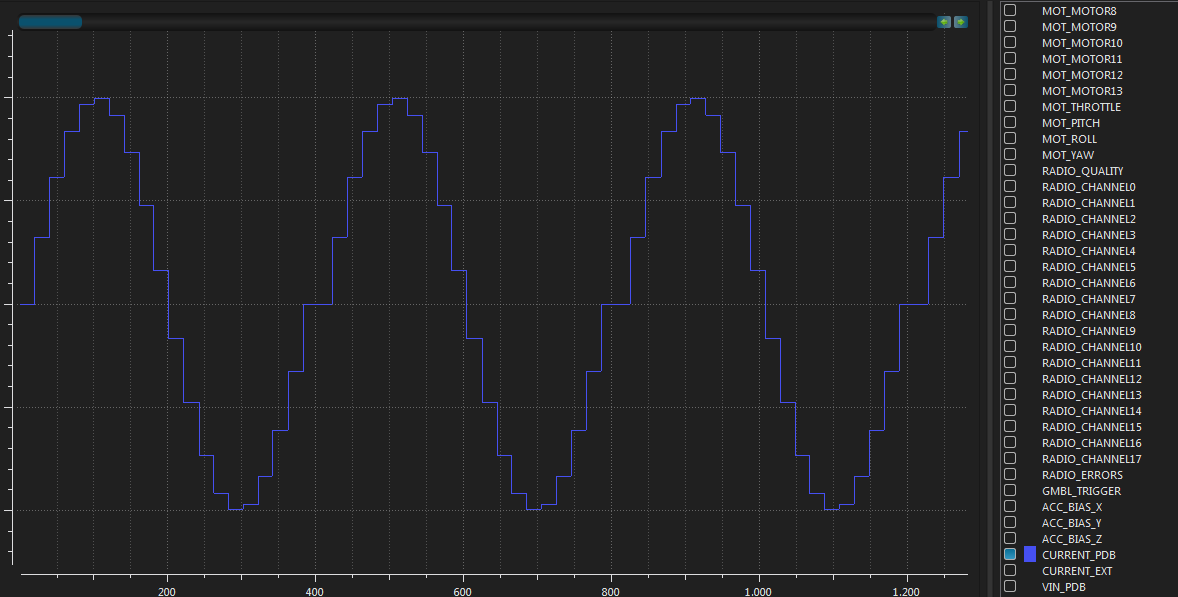
\includegraphics[width=0.8\textwidth]{graphics/test_can_spoof_current.png}
    \caption{Test of python CAN test}
    \label{fig:PCB_block}
\end{figure}
\newpage


\newpage

\section{AutoQuad M4 firmware}
\textbf{AutoQuad} is the flight controller used in this project. The author was among the first students using AutoQuad on SDU, but the first student to make changes to the firmware and to communicate with AQ using CAN-bus. The AutoQuad firmware was not documented at all, so much time was spend reading through code and trying to figure out how it works. A great amount of time was also spend on more practical things like getting to know their Development Environment (CrossWorks for ARM)\footnote{http://www.rowley.co.uk/arm/} in order to compile their firmware, waiting for Quatos\footnote{The controller, Quatos,  used in AutoQuad is not Open Source so a license had to be bought by SDU} license and getting familiar with the flashing process of AutoQuad.\\
Much of the gained knowledge about AutoQuad and how to do debugging has been written down to share with other students. It can be found on the USB-key handed in \textit{Appendix/SDU-UASAutoQuaddocumentation.pdf and SDU-UASAutoQuadsourcecodedocumentation.pdf}. Text marked with green is written by the author.


\textit{Since AutoQuad only supports proving GPS coordinates through a serial port\footnote{Seen by inspection of the schematic to the M4-board done by the supervisor} another way had to be found and implemented.
Sending GPS coordinates through the serial port would require the onboard GPS to be unmounted which seems like a bad solution. The CAN bus was chosen since it is already implemented in AutoQuad. However AutoQuad supports sensor inputs through CAN, GPS was not supported and there by had to be implemented.}

In order to send GPS coordinates to AQ a way in had to be found. A solution would be to unmount the onboard GPS, however that removes the functionality of the M4 board to fly normally without external hardware eg. A RPI. Since AutoQuad gets its coordinates from the onboard ublox M8Q \footnote{\url{http://autoquad.org/wiki/wiki/m4-microcontroller/m4-gps-antenna-options/}} using ublox's ubx protocol, everything sent by eg. a RPI had to be encoded as ubx.
Instead of making hardware changes to the M4 it was decided to use the already supported CAN-bus interface. The M4 board already uses the CAN-bus to send velocities to each of the ESC's on an EduQuad drone. AutoQuad default supports sending some sensor values using the CAN-bus, however GPS coordinates, DOPs and accuracies was not implemented. The only implementation was to receive the battery voltage and current usage and log it to an MicroSD-card.
AutoQuads CAN protocol is described, implemented and tested in section \ref{sec:somewhere}.

When all CAN-nodes has successfully registered, different node-initializing functions run.
First a summary run which sends the number and types of the nodes to QGroundStation. \footnote{Graphical userinterface which provices generel information about the drone such as battery, attitude but also waypoint functionalities}.
It can thus be validated by the pilot that all the ESC's and CAN-sensors are detected.
After the summary, a CAN-sensor initialization happens. The initialization of each CAN-sensor happens which is to send CAN\_CMD\_TELEM\_* described in section \ref{sec:somewhere} but more important also to create a callback.
The callback will then be attached to the CAN-type which in this case is CAN-sensor\footnote{CAN-types are described in section \ref{sec:somewhere}} so when AutoQuad receives a sensor reading the callback will be invoked.\\

Default the callback fills in the sensorvalue in an array so the sensor value can be used in another task. The canID \footnote{Described in section \ref{sec:somewhere}} is then used as index so the task needing the sensorvalue knows where to look since it knows which sensorsvalue it needs. Code \ref{code:callback} shows the callback\footnote{\url{https://github.com/bn999/autoquad/blob/master/onboard/canSensors.c}}
\begin{lstlisting}[language = c, caption = Callback invoked when a CAN-sensorvalue is received. It stores the value in an array indexed by canId, label=code:callback]
void canSensorsReceiveTelem(uint8_t canId, uint8_t doc, void *data) {
    canSensorsData.values[canId] = *(float *)data;

	/* Reception time of the message stored as well */
}
\end{lstlisting}
The callback is fairly simple and does not save the doc\footnote{Described in section \ref{sec:somewhere}} which is needed in order to tell which value the CAN-GPS sensor is sending.\\

All of the CAN-GPS packet handling has been implemented in the callback function. A prettier solution might have been to create a task and use a semaphore to signal when there is a new GPS-packet available. Due to lack of time implementing everything was done in the callback.

Code \ref{code:psudo_parse_can_gps} shows a pseudo code of how the GPS-packets is handled. In section \ref{sec:somewhere} the CAN-GPS packets can be seen.

\begin{lstlisting}[language = Matlab, caption = Modified callback invoked when a sensor-value is received. Shows how doc is used to tell which GPS\-packet is received and when height is received the flags are set, label=code:psudo_parse_can_gps]
canSensorsReceiveTelem(canId, doc, *data) {
	if doc == CAN_DOC_LAT then
		canData.latitude = data
		
	if doc == CAN_DOC_LON then
		canData.longitude = data
		
	if doc == CAN_DOC_DOP then
		canData.xDOP = data[x]
		..
	if doc == CAN_DOC_ACC then
		canData.satellites = data[0]
		canData.fix = data[1]
		canData.xAcc = data[x]
		..
		canData.heading = data[n-1]
		
	if doc == CAN_DOC_VEL then
		gpsData.velx = data[x]
		..		
	if doc == CAN_DOC_ALT then
		gpsDatat.height = data
		if gpsData.fix == 1 and gpsData.satellites >= 8 then
			gpsUpdatetime = now()
			setFlag (gpsData.gpsPosFlag)
			setFlag (gpsData.gpsVelFlag)
		else:
			debug_to_QGroundStation
}
\end{lstlisting}

The \textit{data} pointer given as parameter to the callback is of void pointer. Some pointer gymnastics is done in order to get the right elements from the CAN-packet. If the received CAN-packet is of 8*1 bytes, the void pointer is casted to an uint8\_t pointer so each byte can be retrieved by using the casted pointer as an array. \\

When the flags are set, the task updating the UKF will run \footnote{\url{https://github.com/bn999/autoquad/blob/master/onboard/run.c\#L110} last visited 23 maj}.
Code \ref{code:ukf_update} shows a snippet from the task updating the UKF when the position or velocity flag is set.
\begin{lstlisting}[language = Matlab, caption = Snippet of run.c as psudeocode which updates the UKF when position flag or velocity flag is set, label=code:ukf_update]
if IsFlagSet(gpsData.gpsPosFlag) == yes then
	    navUkfGpsPosUpdate(gpsData.lastPosUpdate, gpsData.lat, gpsData.lon, gpsData.height, ....);
	    ClearFlag(gpsData.gpsPosFlag);
	    
else if IsFlagSet(gpsData.gpsVelFlag) == yes then
	    navUkfGpsVelUpdate(gpsData.lastVelUpdate, gpsData.velN, gpsData.velE, ....);
	    ClearFlag(gpsData.gpsVelFlag);
\end{lstlisting}


\newpage




  can0  00000000   [0] 
  can0  01C00000   [8]  EF BE AD DE 03 09 00 00
  can0  0E000041   [6]  EF BE AD DE 00 00
  can0  14CD0042   [2]  00 08
  can0  14CC0043   [2]  0A 00



seq tæller op så rate/value bliver acknowledged
  can0  00000000   [0] 
  can0  01C00000   [8]  EF BE AD DE 03 09 00 00
  can0  0E000041   [6]  EF BE AD DE 00 00
  can0  14CD0042   [2]  00 08
  can0  00400002   [8]  00 00 00 00 00 00 00 00
  can0  14CC0043   [2]  0A 00
  can0  00400003   [8]  00 00 00 00 00 00 00 00



\section{Indoor localization}
\begin{itemize}
	\item Introduction to section(chapter)
	\item Why use vision as lozalization. cheap, no expensive sensors.
	\item About the MarkerLocator(out of scope), how it works,(Overview - not in depth, why it's slow, how window-mode works) how it's implemented, scalability.
	\item Quality meassure, why is it nessecary.
	\item How I arrived to a good way of meassureing the found marker.
	\item One drone detection
	\item Two drones detection, different ways of detecting orders.
	\item Implementation in ROS, splitting into different nodes.	optimization
\end{itemize}

\begin{figure}[H]
    \center
    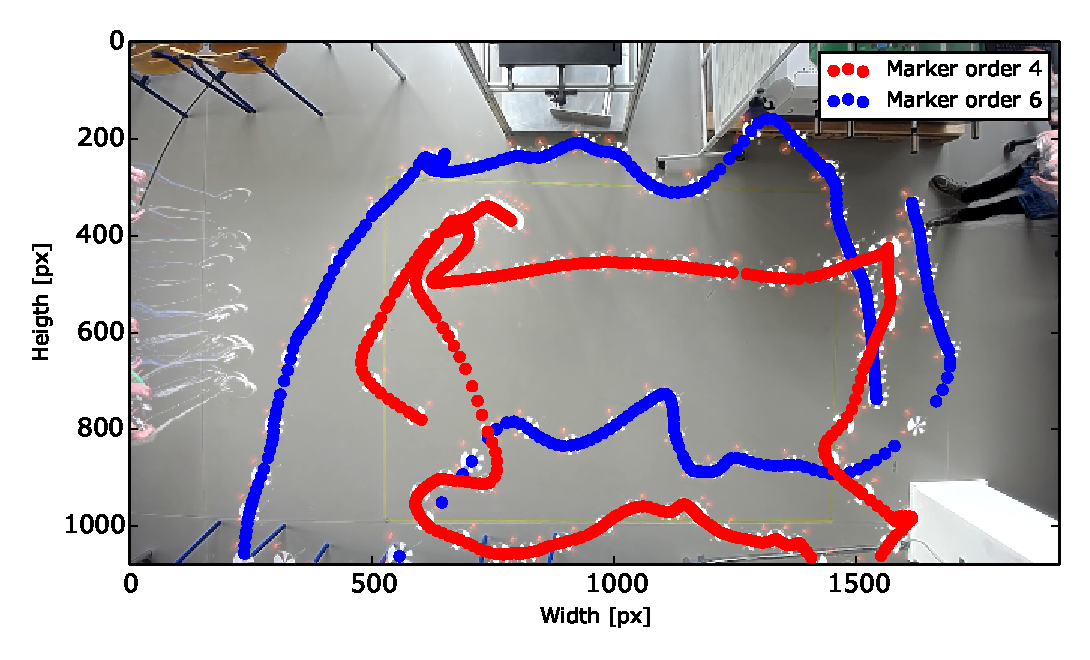
\includegraphics[width=1\textwidth]{graphics/test.eps}
  \label{fig:boat1}
  \caption{Figure showing every 7'th frame merged into one frame combined with the tracked positions of the drones}
\end{figure}
\Mathias{Smaller dot size - almost impossible to see the drone in the frames..}

\Mathias{Red is above blue, not because the drone wasn't detcted}
\Mathias{WIfi test distance, see what happens to latency}

\chapter{Leader-followers}\label{chp:Hardware}
\input{leader-followers}

\chapter{Implementation}
This chapter concerns the most important parts about how this project has been implemented. It has been split into several sections.

\Mathias{Write shortly about the implementation Chapter}
\Mathias{Less calculations on the drone, better to move to another computer/cluster with more power than the drone has available from its battery}
\Mathias{Image of camera and drone seen from the side. Show what happens to the drones position estimation when it drifts down/up}

\section{CAN implementation}
\subsection{Introduction}
In order to spoof the onboard GPS, the CAN-bus was chosen as input to AQ. 
The CAN-bus is already implemented and widely used on a ViaCopter drone to communicate between AQ and hardware like ESCs, PDB etc. Much time was spend reading through the source code and trying to figure out how the protocol works.
The developers behind AQ says, that the code is the documentation and thereby have not written any real documentation. \\
Figuring out how it works was done using debugging utilities such as breakpoints and looking at the content of the different memory locations in CrossWorks.
To further investigate the protocol a PEAK-CAN adapter were connected to a Ladybird drone and several python scripts were developed to send and receive messages from AQ. \\
The author did not go into details about messages used between AQ $\leftrightarrow$ ESC's and AQ $\leftrightarrow$ OSD.\\


\subsection{CAN Protocol description}
A Peak-CAN adapter were used throughout the project. It supports High-speed ISO 11898-2\footnote{\url{http://www.peak-system.com/PCAN-USB.199.0.html?&L=1}} which is a standard that states the properties of physical layer. 
Its max speed is 1 mbit which is the speed AQ uses to communicate on the CAN-bus. 
AQ uses CAN 2.0B which has 29 identifier bits.
AQ is not using an existing protocol on top of ISO 11898-2. The developers created their own to suit their needs.\\

\subsubsection{Identifier bits}
A Generic look at a AQ CAN messages can be seen in table \ref{tab:can_identifier_bits}.
The normal function of the identifier bits is the priority of the messages.
A CAN controller can then be setup to only allow certain messages to be processed depending on their identifier bits.
The identification bits has been split up in AQ to contain information about the sender, receiver etc. Which is not normally saved information in a CAN message.
\begin{table}[H]
\resizebox{\textwidth}{!}{%
	\begin{tabular}{|c|c|c|c|c|c|c|c|}
	\hline
	\multicolumn{8}{|c|}{CAN Message} \\ 
	\hline
	 \multicolumn{7}{|c|}{Identfier bits [29 bits]} &  		\multicolumn{1}{c|}{Data bits [max 64 bits]} \\
	 \hline
	 LCC [28:27] & TT [26] & FID [25:22] & DOC [21:16] & SOID 	[15:11] & TID [10:16] & SEID [5:0] & \\
	\hline
\end{tabular}}
	\caption{Table shows the identifier bits used in AutoQuad CAN messages}
	\label{tab:can_identifier_bits}
\end{table}

In figure \ref{tab:abbri_can_msg} the abbreviations can be seen.
\begin{table}[H]
		\begin{tabular}{|l|l|}
		\hline
		LCC & Logical Communications Channe \\
\hline
		TT & Target Type \\
\hline
		FID & Function ID \\
\hline
		DOC & Data Object Code \\
\hline
		SOID & Source ID \\
\hline
		TID & Target ID \\
\hline
		SEID & Sequence ID \\
\hline
		\end{tabular}
		\caption{Table shows 
abbreviations used in table \ref{tab:can_identifier_bits}}
		\label{tab:abbri_can_msg}
\end{table}

Each of the elements in an AQ messages will be explained how they are used in AQ. \\

\subsubsection{Logic Communication Channel}
LCC is the priority of the message. 
To understand how LCC works, one needs to look into CAN arbitration.
As stated in ISO-11898-2, a 0 is the dominant bit and a 1 is the recessive bit.
The example in figure \ref{tab:can_arbitration} shows two nodes each transmitting a packet.
The arbitration only happens during the transmission of the identifier bits.
In the example on bit 8, Node 16 losses the arbitration and stops transmitting.
Node 15 keeps transmitting its packet because it has lower identifier bits and thereby higher priority.
\begin{figure}[H]
    \center
    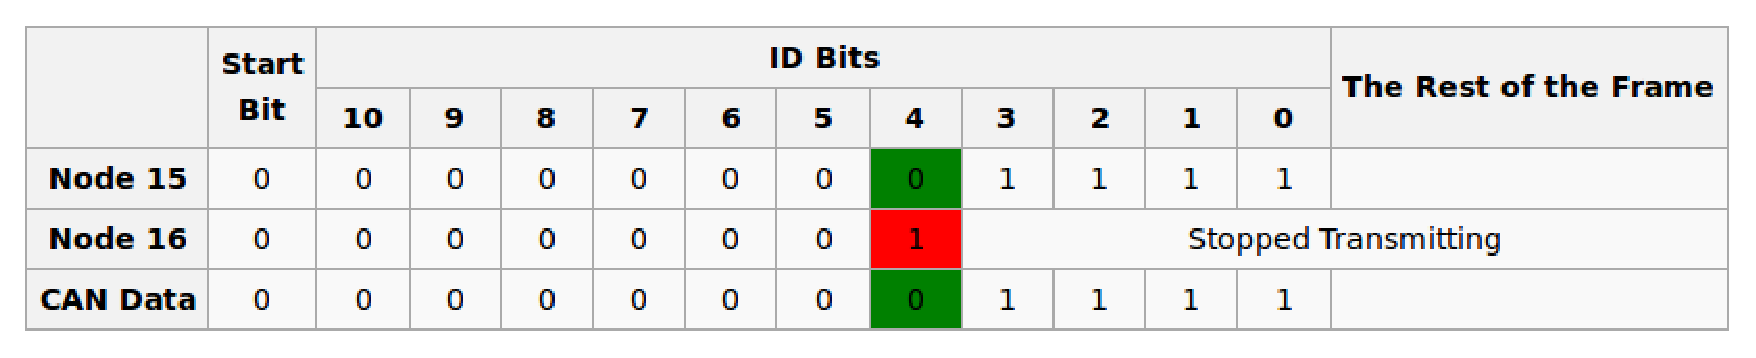
\includegraphics[width=1\textwidth]{graphics/can_arbitration.eps}
    \caption{Example of CAN arbitration where node 15 has the lowest ID and thereby highest priority}
    \label{tab:can_arbitration}
\end{figure}
\newpage
LLC in a message can take one of the defines in code \ref{code:llc_defines}
\begin{lstlisting}[language = c, caption = LLC defines, label=code:llc_defines]
#define CAN_LCC_EXCEPTION   ((uint32_t)0x0<<30)
#define CAN_LCC_HIGH        ((uint32_t)0x1<<30)
#define CAN_LCC_NORMAL      ((uint32_t)0x2<<30)
#define CAN_LCC_INFO        ((uint32_t)0x3<<30)
\end{lstlisting}

\begin{table}[H]
\centering
\caption{Table showing the 4 types of priority in AQ}
\label{my-label}
\begin{tabular}{|l|l|l|}
\hline
\textbf{Name} & \textbf{Value} & \textbf{Priority (lowest first)} \\ \hline
EXCEPTION     & 0000           & 0                 \\ \hline
HIGH          & 0001           & 1                 \\ \hline
NORMAL        & 0010           & 2                 \\ \hline
INFO          & 0011           & 3                 \\ \hline
\end{tabular}
\end{table}

\subsubsection{Target Type}
Target type can either be “node” or “group” depending on if the receiver(s) is one or more nodes. 
\begin{lstlisting}[language = c, caption = Target type defined in AQ, label=code:target_types]
#define CAN_TT_GROUP        ((uint32_t)0x0<<29)
#define CAN_TT_NODE         ((uint32_t)0x1<<29)
\end{lstlisting}
The GROUP is used when AQ sends its reset-msg upon startup.\\
When the authors node send a sensor-measure to AQ it will be of type NODE.
\subsubsection{Function ID}

Function ID describes the function of the CAN message. If it is a PING, ACK, NACK, etc.
It simply states the function of packet so the receiver node knows what to do with the message.
Different types of functions can be seen in code \ref{code:function_defines}
\begin{lstlisting}[language = c, caption = Excerpts from AQ's list of function defines, label=code:function_defines]
#define CAN_FID_RESET_BUS		((uint32_t)0x0<<25)
#define CAN_FID_ACK				((uint32_t)0x1<<25)
#define CAN_FID_REQ_ADDR		((uint32_t)0x7<<25)
#define CAN_FID_GRANT_ADDR	((uint32_t)0x8<<25)
\end{lstlisting}

Table \ref{tab:fid_descriptions} describes the FIDs shown in code \ref{code:function_defines}.
\begin{table}[H]
\centering
\caption{Descriptions of the FIDs mentioned in code \ref{code:function_defines}}
\label{tab:fid_descriptions}
\resizebox{\textwidth}{!}{%
\begin{tabular}{@{}|l|l|@{}}
\toprule
\textbf{FID}          & \textbf{Description}                                                               \\ \midrule
CAN\_FID\_RESET\_BUS  & Message sent by AQ when powered up                                                 \\ \midrule
CAN\_FID\_ACK         & Message sent to AQ when acknowledging a received message                           \\ \midrule
CAN\_FID\_REQ\_ADDR   & Messaged used when a node on the bus tries to register itself as a node on the bus \\ \midrule
CAN\_FID\_GRANT\_ADDR & Messaged sent by AQ when it registers a node as a node on the bus.                 \\ \bottomrule
\end{tabular}
}
\end{table}

Table \ref{tab:fid_descriptions} shows a description of the 4 FIDs used when a node is registered. 

\subsubsection{Data Object Code}
Comming.. Kind of parameter to FID
\Mathias{eksempel på hvordan de bliver brugt i koden - vise function id i switch/case}
\Mathias{Dscripe how the node is created on the BUS}

\subsubsection{Source/Target/Network ID}
When referred to source/target ID but without respect to either sender or receiver but just a CAN-node, then it is referred to as NetworkId. When a node registers itself in AQ, it gets assigned a NetworkId.

\subsubsection{Sequence ID}
The sequence id is incremented on transmission of each message. It is used when eg. 
A CAN-node sends a reply to a get-message, it is then including the sequence id of the get-message so AQ knows what it receives a reply for.

\subsubsection{Data bits}
The data bytes does not have a general definition, it depends on the function id. With some FIDs the data field may contain additional parameters.\\ \\
Eg. When FID is CAN\_FID\_REQ\_ADDR, data has the fields shown in table \ref{tab:packet_from_node}
\begin{table}[H]
\centering
\caption{Packet sent from node when registering in AQ}
\label{tab:packet_from_node}
\begin{tabular}{@{}|c|c|c|c|c|c|c|c|@{}}
\toprule
\multicolumn{8}{|c|}{64 bits}                           \\ \midrule
0 & 0 & CanId & CanType & UUID3 & UUID2 & UUID1 & UUID0 \\
\midrule
7 & 6 & 5 & 4 & 3 & 2 & 1 & 0 \\ \bottomrule
\end{tabular}
\end{table}

\textbf{UUID} is a unique address generated by each node on the bus. In ESC32v2\footnote{\url{https://github.com/bn999/esc32/blob/master/onboard/can.c}} the address is calculated using XXH-hashing algorithm. The algorithm generates a 32 bit hash from a given input value and a salt.
The input to XXH in ESC32v2 is the unique ID that every ARM in the STMF32\footnote{\url{http://www2.st.com/content/ccc/resource/technical/document/reference_manual/59/b9/ba/7f/11/af/43/d5/CD00171190.pdf/files/CD00171190.pdf/jcr:content/translations/en.CD00171190.pdf}}
 family has. Code \ref{code:xxh_canesc32v2} shows how it is implemented in AQ.

\begin{lstlisting}[language = c, caption = Snippet showing UUID generated in ESC32v2, label=code:xxh_canesc32v2]
can.h:20
#define CAN_UUID	0x1FFFF7E8

can.c:753
canData.uuid = XXH32((void *)CAN_UUID, 3*4, 0);
\end{lstlisting}

\textbf{CanType} is the type of the node trying to register. Eq. SENSOR, ESC and SERVO.  \\

\textbf{CanID} is the number of the CanType node trying to register. When an ESC32v2 is trying to register it sends CanId as the ESC number ranging from 1 to the number of ESC's mounted on the drone. The CanID is assign to each ESC manually as part of the configuring.

% redefine the \mess so that \_ works...
\renewcommand{\mess}[4][0]{
  \stepcounter{seqlevel}
  \path
  (#2)+(0,-\theseqlevel*\unitfactor-0.7*\unitfactor) node (mess from) {};
  \addtocounter{seqlevel}{#1}
  \path
  (#4)+(0,-\theseqlevel*\unitfactor-0.7*\unitfactor) node (mess to) {};
  \draw[->,>=angle 60] (mess from) -- (mess to) node[midway, above]
  {#3};
}

\subsection{Registering a node in AQ}

.....
\begin{figure}[H]
    \center
      \begin{adjustbox}{max width=0.5\textwidth}
	\begin{sequencediagram}
	  \newthread{0.4}{pynode}{ROS-node}
	  \newthread{7}{autoquad}{AutoQuad}

	  \mess[1]{autoquad}{CAN\_FID\_RESET\_BUS}{pynode}

	  \begin{call}[3]{autoquad}{Wait(100ms)}{autoquad}
			\postlevel
			\postlevel
			\mess{pynode}{CAN\_FID\_REQ\_ADDR}{autoquad}
			\postlevel
			\mess{autoquad}{CAN\_FID\_GRANT\_ADDR}{pynode}
	  \end{call}
	  \mess{autoquad}{CanTelemeryValue}{pynode}
	  \mess{pynode}{ACKValue*}{autoquad}
	  \postlevel

  	  \mess{autoquad}{CanTelemetryRate}{pynode}
  	  \mess{pynode}{ACKRate}{autoquad}
	\end{sequencediagram}
	\end{adjustbox}
	\label{fig:protocol_req_node}
	\caption{Registering a new node in AQ}
\end{figure}

Test of sending sensor data
\begin{figure}[H]
    \center
    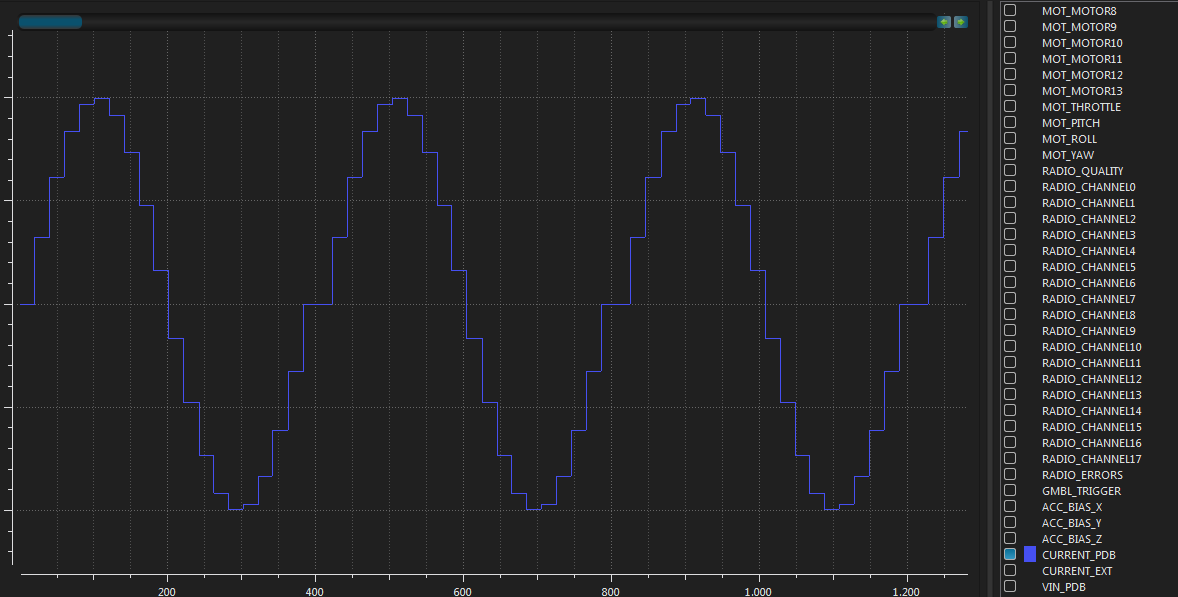
\includegraphics[width=0.8\textwidth]{graphics/test_can_spoof_current.png}
    \caption{Test of python CAN test}
    \label{fig:PCB_block}
\end{figure}
  can0  00000000   [0] 
  can0  01C00000   [8]  EF BE AD DE 03 09 00 00
  can0  0E000041   [6]  EF BE AD DE 00 00
  can0  14CD0042   [2]  00 08
  can0  14CC0043   [2]  0A 00



seq tæller op så rate/value bliver acknowledged
  can0  00000000   [0] 
  can0  01C00000   [8]  EF BE AD DE 03 09 00 00
  can0  0E000041   [6]  EF BE AD DE 00 00
  can0  14CD0042   [2]  00 08
  can0  00400002   [8]  00 00 00 00 00 00 00 00
  can0  14CC0043   [2]  0A 00
  can0  00400003   [8]  00 00 00 00 00 00 00 00


\section{Communication flow}
\begin{table}[H]
\centering

\begin{tabularx}{0.75\textwidth}{@{}|X|X|X|X|X|X|@{}}
\toprule
Content & Lat    & Lon    & Height & DOP   & CRC-16  \\ \midrule
Datatype    & double & double & float  & float & uint16\_t \\ \midrule
Bytes    & 31:24  & 23:16   & 15:8    & 7:4 & 3:0 \\ \bottomrule
\end{tabularx}
\Mathias{Ændre 0:3 til 0:1 da en uint16\_t kun tager 2 bytes og ikke 4}
\caption{Message sent from PC to ESP8266}
\label{my-label}
\end{table}

\section{Vision based localization}
\begin{itemize}
	\item Introduction to section(chapter)
	\item Why use vision as lozalization. cheap, no expensive sensors.
	\item About the MarkerLocator(out of scope), how it works,(Overview - not in depth, why it's slow, how window-mode works) how it's implemented, scalability.
	\item Quality meassure, why is it nessecary.
	\item How I arrived to a good way of meassureing the found marker.
	\item One drone detection
	\item Two drones detection, different ways of detecting orders.
	\item Implementation in ROS, splitting into different nodes.	optimization
\end{itemize}

\begin{figure}[H]
    \center
    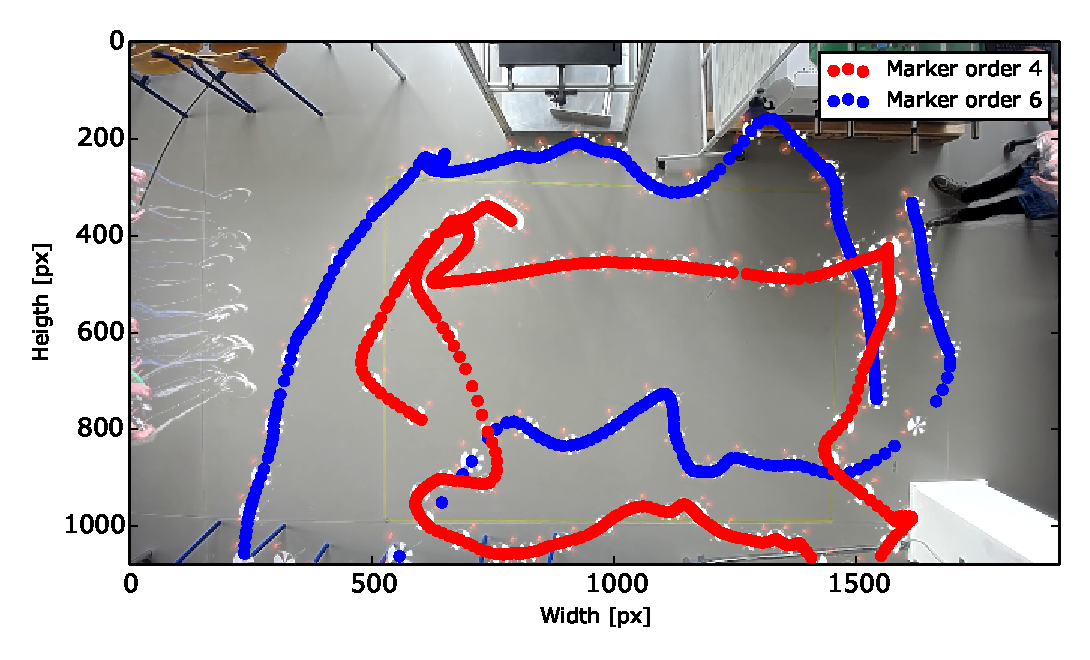
\includegraphics[width=1\textwidth]{graphics/test.eps}
  \label{fig:boat1}
  \caption{Figure showing every 7'th frame merged into one frame combined with the tracked positions of the drones}
\end{figure}
\Mathias{Smaller dot size - almost impossible to see the drone in the frames..}

\Mathias{Red is above blue, not because the drone wasn't detcted}
\Mathias{WIfi test distance, see what happens to latency}
\newpage

\section{Software}
\textit{This capter concerns only the Atmega.  The ESP module will be descriped in section \ref{sec:esp_firmware}} \\
In order to have a timing on the At90CAN128 a scheduler was chosen and implemented.
The list below shows 3 different types of scheduler that was considered.
\begin{itemize}
	\item Real-time Operating System(RTOS) provides strict timing but at the cost of overhead. A RTOS runs task in a "parallel" environment. Each task runs in a loop and the RTOS scheduler will do context switching when needed. Using a RTOS requires mutexes and semaphores to protect shared resources which increases the complexity and amount of overhead
	\item Super-Loop provides no timing at all, but process data as fast as possible. It does not do any context switching and does not require mutexes or semaphores and  and thereby takes no overhead.
	\item Run-To-Complete(RTCS) scheduler is a mix of the two other schedulers. It works by waiting for a tick generated by a hardware timer and then starts executing all tasks from the beginning. The order of the task matters if there is dependency between the tasks but also to make sure the task requiring the most precise timing is at the beginning of the list of the tasks. All tasks have to be finished executing before the next tick is giving in order to avoid timing is ruined.
\end{itemize}
The RTCS was chosen since it provides timing without the overhead created when doing context-switching and the need of mutex and semaphores. It further reduces the code-complexity.\\

\Mathias{A little description about the scheduler implementation. Add tasks, and run the scheduler. Show how it waits for tick and the runs through all of the tasks that is in RUN state.}

It was decided to implement the code in tasks to make a low coupling between the functionalities. This makes it easier to maintain and expand later of if needed. The task diagram shown in figure \ref{fig:task_diagram_atmega} shows the tasks and how they do intertask communication.


\begin{figure}[H]
    \center
    \includegraphics[width=0.9\textwidth]{graphics/task_diagram.png}
  \caption{Tasks diagram showing overview of the running tasks on the At90Can128}
    \label{fig:task_diagram_atmega}
\end{figure}
A small description of each of the tasks is given below:
\begin{itemize}
\item \textbf{ is\_alive\_task} Toggles the green led to make sure the scheduler is running. In case of stack overflow, memoryleak or any other error, the Atmega will freeze and it will easily be detectable since the green led stops blinking
\item \textbf{ uart0\_tx\_task} Responsible of sending characters in the uart0\_tx queue.
\item \textbf{ uart0\_rx\_task} Responsible of checking if any characters in the uart-receive buffer is available. If any, put them into the uart0\_rx queue
\item \textbf{ uart1\_tx\_task} Responsibile as uart\_0\_tx\_task
\item \textbf{ uart1\_rx\_task} Responsibile as uart\_0\_rx\_task
\item \textbf{ can\_rx\_task} Responsible of checking if a CAN-message is available in the MOB. If any put them into the CAN\_rx\_queue
\item \textbf{ can\_tx\_task} Responsible of transmitting messages available in the CAN\_tx\_queue
\item \textbf{ aq\_node\_task} Responsible of registering the node when AQ boots.
\item \textbf{ task\_slip\_decode\_crc\_task} Responsible of removing SLIP characters and run CRC
\item \textbf{ aq\_spoof\_task} Responsible of converting and transmitting received GPS messages from uart1.
\end{itemize}
\Mathias{Add description of slip and crc task, maybe also spoof and node, not sure..}

\subsubsection*{Test of RTCS timing}
In order to test the timing of the scheduler, a led\_task was written. The task can be seen in code \ref{code:test_scheduler}
\begin{lstlisting}[language = c, caption = RTCS task used in timing test, label=code:test_scheduler]
void is_alive_task(uint8_t my_state){

	// Write to UART0
	UDR0 = my_state+'0';

	switch(my_state){
	case 0:
		INT_LED_ON_GREEN;
		INT_LED_OFF_RED;
		INT_LED_OFF_BLUE;
	    set_state( 1 );
		break;
	case 1:
		INT_LED_OFF_GREEN;
		INT_LED_ON_RED;
		INT_LED_OFF_BLUE;
	    set_state( 2 );
		break;
	case 2:
		INT_LED_OFF_GREEN;
		INT_LED_OFF_RED;
		INT_LED_ON_BLUE;

		// Set next state
	    set_state( 0 );
		break;
	}
	// Wait one second
	wait( 1000 );
}
\end{lstlisting}

The test was done by writing the current state of the task to UART0.\\ A python script were made that measures the time between each character received. The script can be seen in code \ref{code:test_rtcs_python}.
\begin{lstlisting}[language = python, caption = Python code used to measure time between received byte, label=code:test_rtcs_python]
#!/usr/bin/python
import serial
import time

ser = serial.Serial( port='/dev/ttyUSB0', baudrate=57600 )

t = time.time()
while True:
    char =  ser.read(1):
    print time.time() - t, ","
    t = time.time()

ser.close()
\end{lstlisting}
The output of the script were redirected to a file. After receiving 700 bytes the standard deviation and mean was calculated using matlab.
The mean is 1.0089 sec with a standard deviation of 0.0042 sec.

Part of the variance is caused by the inaccuracy of the timing on the PC running the python code. If a more accurate measure was needed, a scope could be attached to the $\mu$C's GPIO. Each time the scheduler enters the task the GPIO should be set high, and when it exists the GPIO should be set low. The scopes at SDU is capable of telling the variance of the off signal. \\
It can be concluded that the scheduler performs well.
\section{Hardware}
\subsection{Introduction}
This secion will go in depth about the extentionboard created as ab addon to the AQ M4 board. The extentionboard was developed to act as a bridge between PC and the CAN-bus using wireless communication in order to send GPS coordinates from the PC to the Drones.\\

The block schematic shown in figure \ref{fig:PCB_block} was created by the auther of the report. It was then given to Carsten Albertsen who created the schematic and did rest of the creation of the PCB.
\\
\Mathias{Create schematic appendix}
\Mathias{Add GPS, WIFI, PCB, PC to forkortelses liste}
\Mathias{Thanks to Carsten Albertsen for PCB development}
\begin{figure}[H]
    \center
    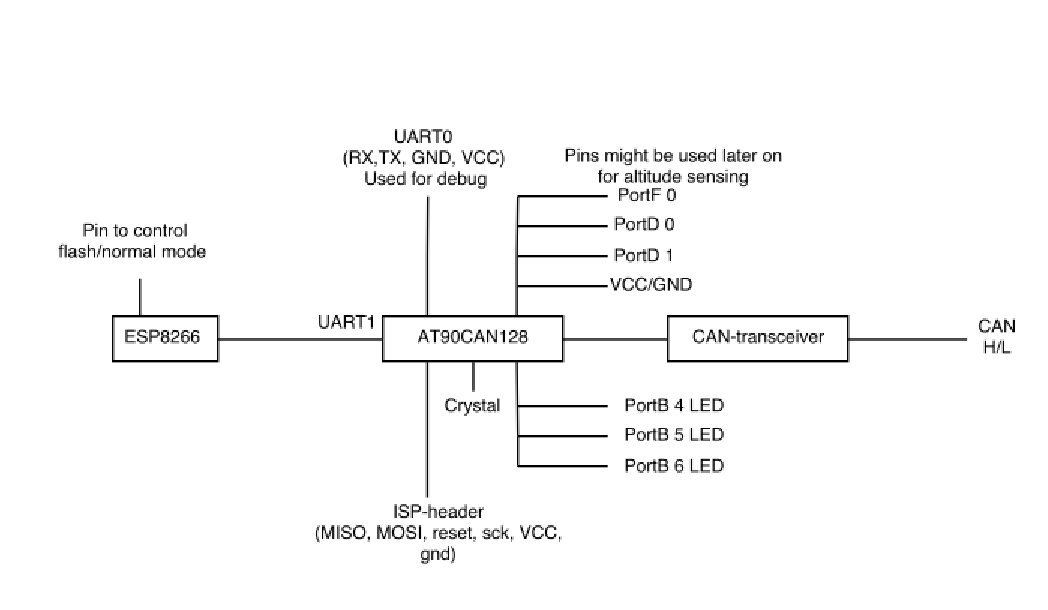
\includegraphics[width=1\textwidth]{graphics/PCB_block_v3.eps}
    \caption{Block schematic of the WIFI-extentionboard developed to AQ M4}
    \label{fig:PCB_block}
\end{figure}

\subsubsection{ATmega}
\subsubsection{Wireless Communication}
An important part of the hardware is the wireless communication used between the PC and the drones.
The wireless communication mpodule has severel requirements it needs to fulfill in order to make the whole system work as expected. A comparesiontable has been made in table \ref{tab:compare_table_wireless_communication} to find the wireless communication module that is best suited for the task.


\begin{table}[H]
	\centering
	\begin{tabular}{@{}|l|l|l|l|l|l|l|@{}}
		\toprule
		\textbf{Product} & \textbf{Size} & \textbf{Price} & 				\textbf{Usability} & \textbf{Power consumption} & 					\textbf{Range} & \textbf{Score} \\ \midrule
		ESP8266          &               &                &                    		&                            &                &                		\\ \midrule
		EMW3165          &               &                &                    		&                            &                &                		\\ \midrule
		nRF51822         &               &                &                    		&                            &                &                		\\ \bottomrule
	\end{tabular}
	\caption{Comparisontable used to compare different wireless 		communication modules}
	\label{tab:compare_table_wireless_communication}
\end{table}

\subsubsection{Pins}
A few pins where made available through solder pads for easy access if needed later on.

The following pins where available as solder pads:
\begin{itemize}
	\item PortF 0 - Alternative function as ADC, channel 0
	\item PortD 0 - Alternative function as interrupt, INT0
	\item PortD 1 - Alternative function as interrupt, INT1
\end{itemize}
In case the onboard baromter isn't accurate enough, an alternative distance could be used to measure the drones altitude with respect to the ground.
PortF0 has been made available since some distance sensors give output as an analogue value. 
An example of such sensor is an Infrared proximity sensor.\footnote{http://www.sharpsma.com/webfm\_send/1208} \\
As an alternative type of distance sensor, a ultrasoinc could be used such as HCSR04.
As output it gives a binary output with high-time proportional with the distance.\footnote{http://www.micropik.com/PDF/HCSR04.pdf}.
To detect the high-time, one of PortD1/0 would be useful. \\

Which type of sensor suits best as a distance sensor to provice altitude information to the drone is ouf of the scope of this report. The PCB has just been made ready to different types of sensors.

\subsubsection{Debug/ISP}
In the final schematic UART0 and ISP pins where combined in one pinheader for easy access through one cable. \Mathias{Refer to image of board}
To program the AtMega the ISP pins where required to be easy accessable. 
UART0 was made accessable to be used as debug and programming of the ESP8266 board.
The plan was to setup the AtMega as UART passthrough from UART0 to UART1.
Due to a mistake\footnote{The wrong pair of MISO/MOSI pins where made available in the ISP-header. The correct pair of MISO/MOSI is also RXD0/TXD0 as alternative function} in the final schematic, both UART0 and UART1 where made accessable trough the ISP/debug header. 
This ended up making it easier to program the ESP8266-board without using the AtMega as UART passthrough.

\newpage

\chapter{Test Descriptions}
\Mathias{Maybe a chapter called "Test Descriptions here"}
%\input{test_descriptions}

\chapter{Results}\label{chp:Hardware}
\input{results}

\chapter{Discussion}\label{chp:Hardware}
\input{discussion}

\chapter{Conclusion}\label{chp:Hardware}
\input{conclusion}


\chapter{Future work}\label{chp:Hardware}
\begin{itemize}
	\item Autodetect drones using avahi/mDNS. Instead of specificing the ID and ipaddress of each drone in the launch file, it could be handled automatically by avahi.
\end{itemize}


% --------- End Matter --------- %

\newpage
\listoffigures
%\begingroup
%\let\clearpage\relax
\newpage
\listoftables
%\endgroup

\begin{appendices}
\makeatletter
\addtocontents{toc}{\let\protect\l@chapter\protect\l@section}
\makeatother
\makeatletter
\addtocontents{toc}{\let\protect\l@section\protect\l@subsection}
\makeatother
\addtocontents{toc}{\protect\setcounter{tocdepth}{1}} % Exclude everthing from \section and downwards from ToC
\captionsetup{list=no} % Exclude all figures and tables from LoF and LoT

% Chapter 2 Hardware:
% Chapter 3 Vision:
%\input{app_camera_calibration}
%\input{app_evs_object_detection}
%\input{app_distance_calculation}
%\input{app_opencv_functions}
%\input{app_canny_edge}

% Chapter 4 Communication:
%\input{app_dual_rpi_speed}
%\input{app_K827P_speed}

% Chapter 5 UR5 Controller System:
%\input{app_final_implementation_benchmark}


\end{appendices}

%\bibliographystyle{siam}
%\bibliography{bibliography}
\printbibliography

\end{document}
